In this section, we empirically validate the theoretical result proved in \Cref{sec:theory}. We again consider the linear bandit setting discussed in \Cref{sec:short-horizon}. Recall that the linear bandit setting consist of horizon $n=25$, $\Mpr = \{100000, 200000\}$, $\Mts = 200$, $A=10$, and $d=2$. 
%
%
The demonstrator $\pi^w$ is the \ts\ algorithm and we observe that \pred\ (\gt) has lower cumulative regret than \dptg, \ad\ and matches the performance of \linucb. 

\textbf{Baseline (\linucbt):} We define soft LinUCB (\linucbt) as follows: At every round $t$ for task $m$, it calculates the ucb value $B_{m,a,t}$ for each action $\bx_{m,a} \in \X$ such that $B_{m,a,t} = \bx_{m,a}^\top \wtheta_{m,t-1} + \alpha\|\bx_{m,a}\|_{\bSigma_{m,t-1}^{-1}}$ where $\alpha > 0$ is a constant and $\wtheta_{m,t}$ is the estimate of the model parameter $\btheta_{m, *}$ at round $t$. 
%
Here, $\bSigma_{m,t-1} = \sum_{s=1}^{t-1}\bx_{m,s}\bx_{m,s}^\top +\lambda\bI_d$ is the data covariance matrix or the arms already tried.
%
Then it chooses $I_t \sim \mathrm{softmax}_a^\tau(B_{m,a,t})$, where $\mathrm{softmax}_a^\tau(\cdot)\in\triangle^A$ denotes a softmax distribution over the actions and $\tau$ is a temperature parameter (See \Cref{sec:short-horizon} for definition of $\mathrm{softmax}_a^\tau(\cdot)$).

\textbf{Outcomes:} We first discuss the main outcomes of our experimental results:

\begin{tcolorbox}
\customfinding \pred\ (\gt) excels in predicting the rewards for test tasks when the number of training (source) tasks is large. 
\end{tcolorbox}

% \noindent
% \textbf{(1)} The \pred\ (\gt) excels in predicting the rewards for test tasks when the number of training (source) tasks is large. 

% \textbf{(2)} The \pred\ (\gt) has a poor prediction of the rewards for test tasks when the number of training (source) tasks is small. 


% \begin{figure}[!hbt]
% \centering
% \begin{tabular}{ccc}
% \subfigure[Prediction Error for $100000$ tasks]{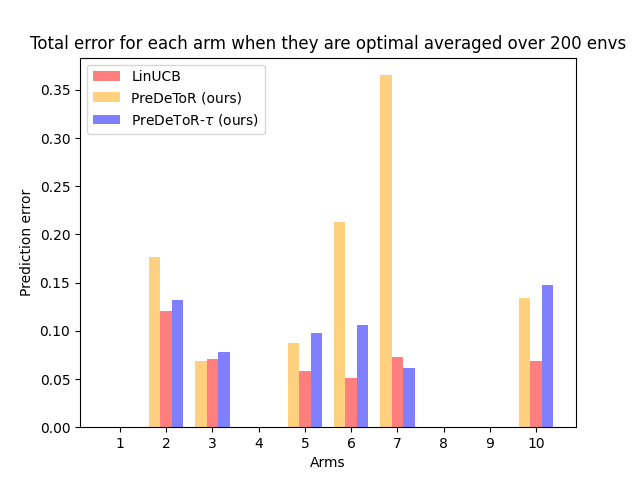
\includegraphics[scale = 0.27]{img/Neurips/linear/analysis_total_smaller_train_env.png}\label{fig:prediction-error-small}} &
% %%%%%%%%%%
% \subfigure[Prediction Error for $200000$ tasks]{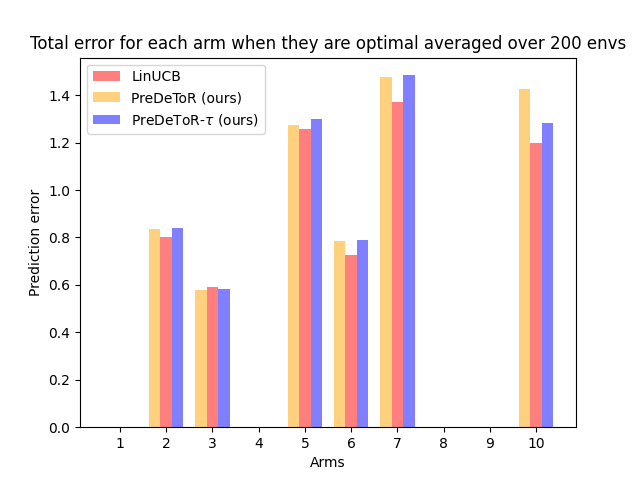
\includegraphics[scale = 0.27]{img/Neurips/linear/analysis_total.png} \label{fig:prediction-error-large}} &
% %%%%%%%%%%
% \subfigure[Cumulative Regret of \pred\ (\gt) compared against \linucbt]{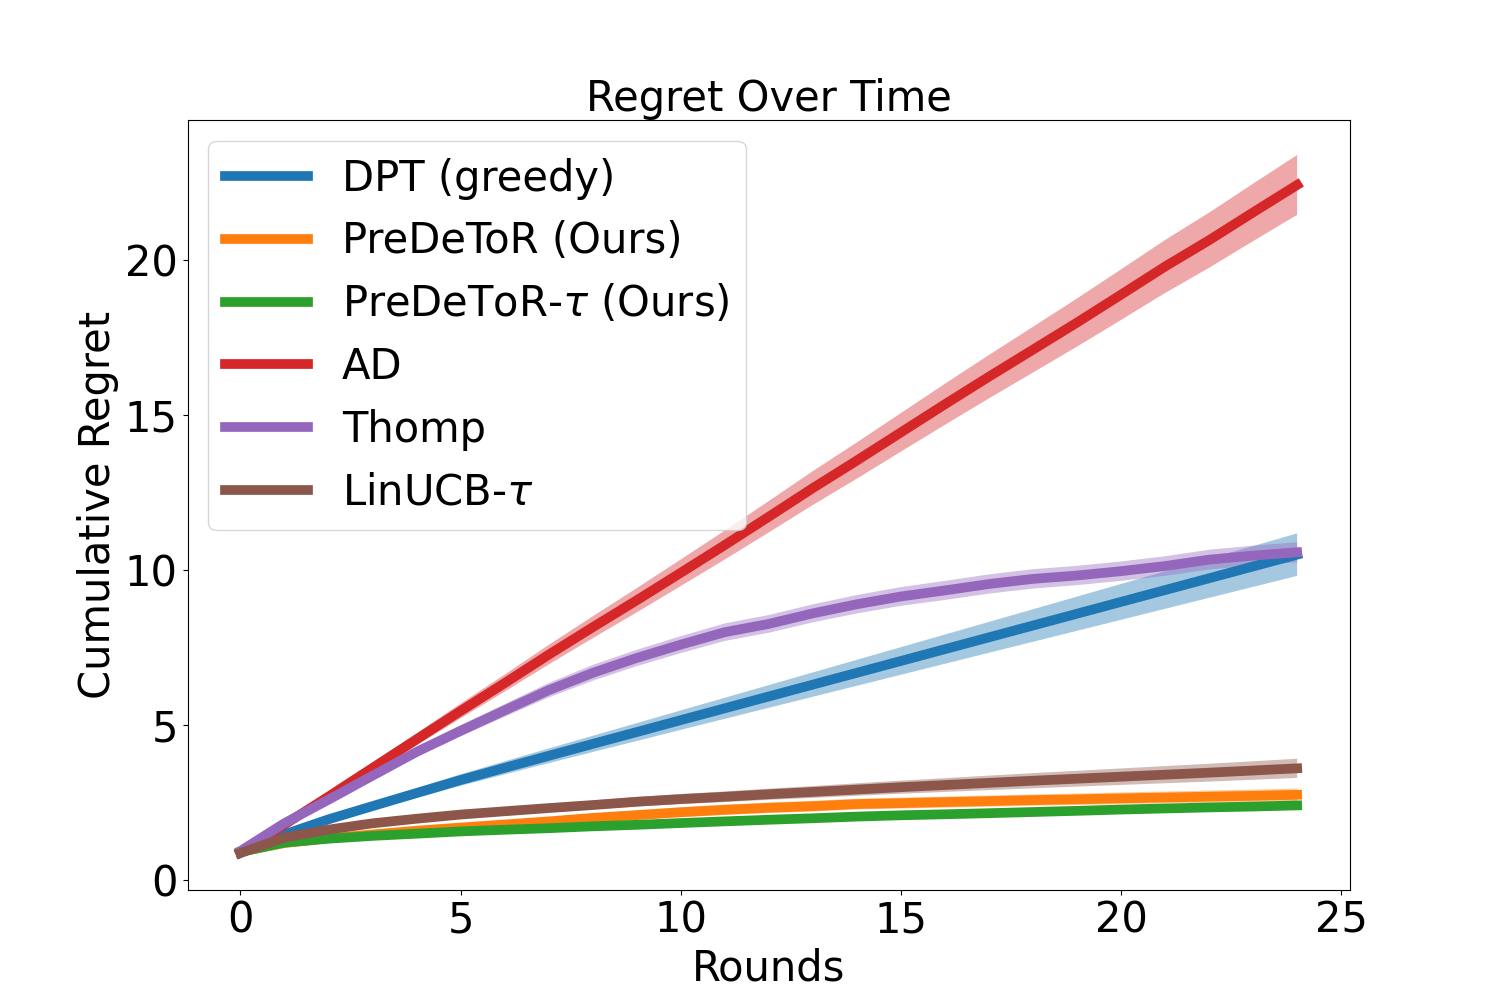
\includegraphics[scale = 0.13]{img/Neurips/theory/lin_tau_lr0.00015_do0_embd32_layer4_head4_envs100009_hists1_samples1_var0.3_cov0.0_H25_d10_lind2_seed1_testcov0.0_hor25.pkl.png} \label{fig:comparison-with-linucb}}
% \end{tabular}
% \caption{Empirical validation of theoretical analysis}
% \label{fig:empirical-validation}
% \end{figure}

\begin{figure}[!hbt]
\centering
\begin{subfigure}[b]{0.32\textwidth}
   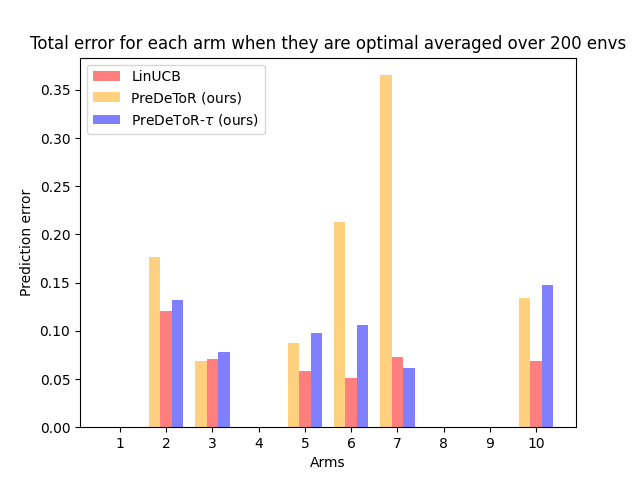
\includegraphics[scale=0.27]{img/Neurips/linear/analysis_total_smaller_train_env.png}
   \caption{Prediction Error for $10^5$ tasks}
   \label{fig:prediction-error-small}
\end{subfigure}%
\begin{subfigure}[b]{0.32\textwidth}
   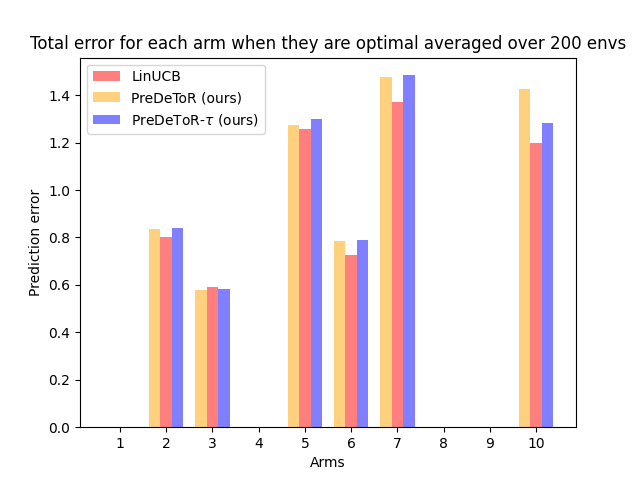
\includegraphics[scale=0.27]{img/Neurips/linear/analysis_total.png}
   \caption{Prediction Error for $2\times 10^5$ tasks}
   \label{fig:prediction-error-large}
\end{subfigure}%
\begin{subfigure}[b]{0.32\textwidth}
   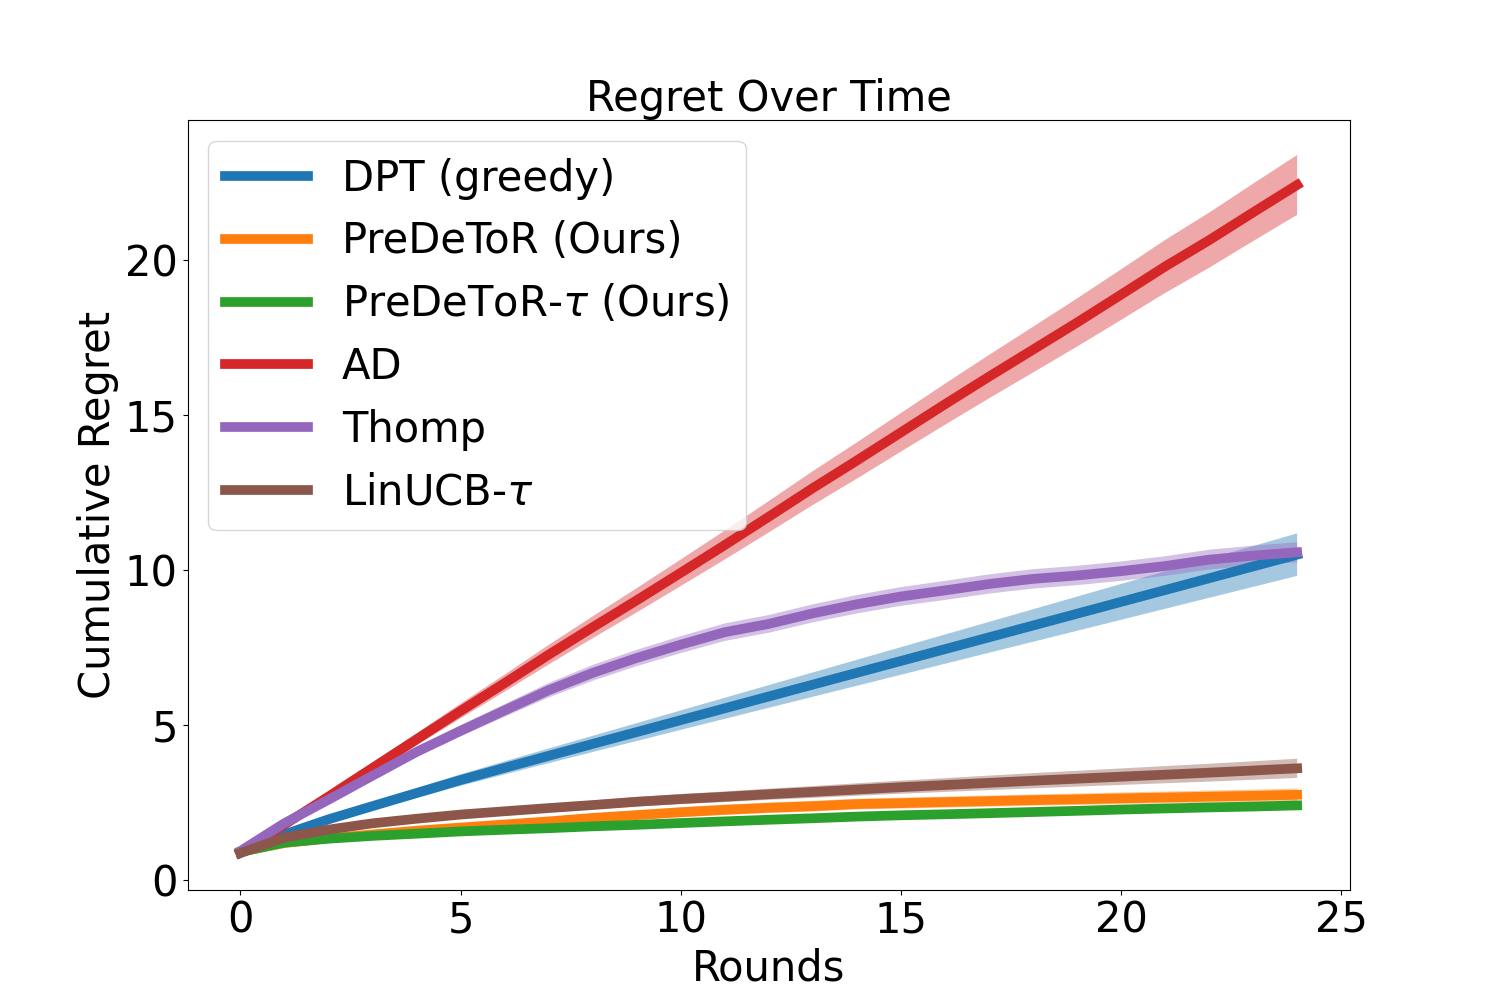
\includegraphics[scale=0.13]{img/Neurips/theory/lin_tau_lr0.00015_do0_embd32_layer4_head4_envs100009_hists1_samples1_var0.3_cov0.0_H25_d10_lind2_seed1_testcov0.0_hor25.pkl.png}
   \caption{Cumulative Regret of \pred\ (\gt) compared against \linucbt}
   \label{fig:comparison-with-linucb}
\end{subfigure}
\caption{Empirical validation of theoretical analysis}
\label{fig:empirical-validation}
\end{figure}

\textbf{Experimental Result:} These findings are reported in \Cref{fig:empirical-validation}.
%
In \Cref{fig:prediction-error-small} we show the prediction error of \pred\ (\gt) for each task $m\in[\Mts]$. The prediction error is calculated as $(\wmu_{m,n, *}(a) - \mu_{m, *}(a))^2$ where $\wmu_{m,n, *}(a) = \max_a\wtheta_{m,n}^\top\bx_m(a)$ is the empirical mean at the end of round $n$, and $\mu_{*,m}(a)=\max_a\btheta_{m,*}^\top\bx_m(a)$ is the true mean of the optimal action in task $m$. Then we average the prediction error for the action $a\in [A]$ by the number of times the action $a$ is the optimal action in some task $m$. We see that when the source tasks are $100000$ the reward prediction falls short of \linucb\ prediction for all actions except action $2$.

In \Cref{fig:prediction-error-large} we again show the prediction error of \pred\ (\gt) for each task $m\in[\Mts]$ when the source tasks are $200000$. Note that in both these settings, we kept the horizon $n=25$, and the same set of actions. We now observe that the reward prediction almost matches \linucb\ prediction in almost all the optimal actions.


In \Cref{fig:comparison-with-linucb} we compare \pred\ (\gt) against \linucbt\ and show that they almost match in the linear bandit setting discussed in \Cref{sec:short-horizon} when the source tasks are $100000$. 